\documentclass[twocolumn]{article}
\usepackage[utf8]{inputenc}
\usepackage{amsmath} % Advanced math typesetting
\usepackage[utf8]{inputenc} % Unicode support (Umlauts etc.)
\usepackage[english]{babel} % Change hyphenation rules
\usepackage{hyperref} % Add a link to your document
\usepackage{graphicx} % Add pictures to your document
\usepackage{listings} % Source code formatting and highlighting
\usepackage{bookmark}
\usepackage{natbib}
\usepackage{geometry}
\usepackage{bbm}
%\usepackage{multicol}
\usepackage{fancyhdr}
\usepackage[document]{ragged2e}
\usepackage{adjustbox}
\usepackage{subcaption}
% \pagestyle{fancy}
% \fancyhf{}
% \fancyhead[LE,RO]{Overleaf}
% \fancyhead[RE,LO]{Guides and tutorials}
% \fancyfoot[CE,CO]{\leftmark}
% \fancyfoot[LE,RO]{\thepage}
\graphicspath{ {Immagini/} }
%C:\Users\erikz\OneDrive\Desktop\PaioPaio2\IMM-Sensors-Network\Latex\Immagini
\geometry{
 a4paper,
 total={170mm,257mm},
 left=20mm,
 top=20mm,
 }

\title{Report and analysis on implementation of IMM algorithm for multiple-model dynamics tracking}
\author{
Paiola Lorenzo 198573 

Zanolli Erik 198852}
\date{January 2020}





\begin{document}

\maketitle



\section*{Introduction}
\justify
The purpouse of this project is to analyze and evaluate the performance of an IMM algorithm's implementation in a distributed environment for
multiple-model dynamics tracking as the tracked agent switches between linked models of movement by the means of a Markov chain. The goal 
is to evaluate the best trade-off between error on estimated position and real position and number of messages regarding consensus involved in the tracking.


    \section*{Setting}
    \justify
    The general objective of this report is to provide a robust tracking that works in a distributed manner for some object that can move 
    in a number of different ways (modelized as a set of dynamical systems $\mathbbm{M}$). The environment in which this object moves is 
    one of a large room that contains multiple sensors that can talk to each other.
    \\
    \subsection*{Sensor's model}
    The sensors chosen are radars measuring the polar cordinates relative to themselves at which the agent is collocated at the timestep, and
    are disposed in a uniform square grid. In order to simulate the real workings of a sensor, range of measuremnt has been limited to the distance
    between one sensor and the following one in any direction of the grid, as soon as the agent exceed the imposed maxiumum distance from the sensor,
    the device will stop sensing.
    This property of the sensor grid, coupled by its geometry, ensures that no more than 4 sensors can measure the agent position at any time,
    so it made sense to let the sensors switch between 3 different states named ON, OFF and IDLE. This can be justified as a way to make the system
    more power efficient and to avoid useless data stream towards sensors that aren't currently in range and sensing.
    The sensor is modeled as a state machine as shown in figure \ref{fig:statemachine}
    \\
    \begin{figure}[h!]
        \centering
        \includegraphics[width=\columnwidth]{sensor_state_machine.png}
        \caption{State machine sensor}
        \label{fig:statemachine}
    \end{figure}
    \\
Sensors in different states differ between each other by the actions that are allowed in the state they are currently in.
\\
Here we enumerate such allowed actions:
\begin{itemize}
    \item ON: at each time-step checks if it is still in range with the function inRange(), takes a measurement, computes the IMM algorithm and 
             at a tunable rate computes the consensus with the other nearby ON sensors. If it's not in range anymore then turns IDLE.
    \item IDLE : checks if it is now in range with the function inRange(), if it is then initialize itself with the data from nearby sensors 
                that are ON. If it recieves a CantSense signal, it checks if at least one of its neighboors is still ON, else it turns OFF itself.
    \item OFF : does nothing but waits for a CanSense signal sent by a neighboor and turns IDLE in the case it has received one (this means that 
                a nearby sensor has turned ON).
\end{itemize}
    So sensors can communicate with the devices adjacent to them (Neighboorhood), as represented in the figure \ref{fig:neighboors} below, 
    and exchange with them signals named CanSense and CantSense which state respectively whenever the agent gets in or goes out of the 
    communicating sensor's range. This check is done through the function inRange() that also serves as a switch between the states of the 
    sensor, as already shown by the figure \ref{fig:statemachine} above.
    The messages that the sensors exchange with their Neighboorhood are
\begin{itemize} 
    \item CanSense : message sent by a sensor switching from IDLE to ON triggered by a positive result from InRange() function
    \item CantSense : message sent by a sensor switching from ON to IDLE triggered by a negative result from InRange() function
\end{itemize}
    \begin{figure}[h!]
        \centering
        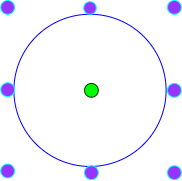
\includegraphics[width=0.2\textwidth]{Immagini/2sensor.png}
        \caption{The neighboors of a sensors are the one immediately adiacent, represented as purple in this image}
        \label{fig:neighboors}
    \end{figure}
    By defing the range of the sensors equal to their spacing on the grid it follows that only a maximum of 4 sensors can be turned on. 
    This fact is shown in the following picture that illustrates the different cases
    \begin{figure}[h!]
        \centering
        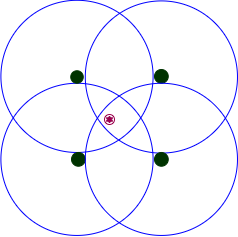
\includegraphics[width=0.23\textwidth]{Immagini/4sensor.png}
        \caption{}
        \label{fig:number}
    \end{figure}
    \begin{itemize}
        \item blue : 1 sensors ON, happens only at the conrners of the grid
        \item yellow : 2 sensors ON 
        \item orange : 3 sensors ON 
        \item red : 4 sensors ON 
    \end{itemize}
    Whenever the target is in range of a sensor at given timestep, the device takes a measurement.
    The model choosen for our sensor is a Radar, and as such the non-linear measurement function
     associated to it is the cartesian to polar transformation at timestep $k$, as shown below
    \begin{align*}
        &z(k)=h(x(k))+v(k)\\
        &\begin{bmatrix}
            \rho(k)\\ \theta (k)(k)
        \end{bmatrix}=  
        \begin{bmatrix}
            \sqrt{x_{1}(k)^2+x_{2}(k)^2}\\ atan2(x_{2}(1)/x_{1}(k))
        \end{bmatrix} +
        \begin{bmatrix}
            v_{1}(k)\\v_{2}(k)
        \end{bmatrix}
    \end{align*}
    where $h(x)$ is the polar to cartesian cordinates transform that takes in $x(k)$ that is the state (of which the first 2 elements are the cartesian
    cordinates relative to the sensor), $z(k)$ is the measure and $v(k)$ is the noise associated to the measurement's operation. The measurement noise $w(k)$ is associated 
    to a diagonal power spectral density matrix $R$.
    \begin{equation*}
        R=\begin{bmatrix}
            \sigma^{2}_{\rho}&0\\
            0&\sigma^{2}_{\theta (k)}
        \end{bmatrix}
    \end{equation*}
    \\
   The matrix $H^{k}=(\nabla_{x} h(x))_{|x=x(k)}$ used in the linearized model with $v(k)=0$, necessary in the IMM filter at each timestep $k$,
   computes to 
    \begin{equation*}
        H^{k}= \begin{bmatrix}
            \frac{x_{1}}{\sqrt{x_{1}^{2}+x_{2}^{2}}} & \frac{x_{2}}{\sqrt{x_{1}^{2}+x_{2}^{2}}}& 0 \dots\\
            \frac{-x_{2}}{x_{1}^{2}+x_{2}^{2}}  & \frac{x_{1}}{x_{1}^{2}+x_{2}^{2}}& 0 \dots\\
        \end{bmatrix}_{|x(k)}
    \end{equation*}
    Where $0\dots$ is a vector of zeroes for all the other states that do not influence the measurement function.
  
    \section*{Model used}
    As mentioned already, the agent we want to track has a variable-model dynamic that can switch between different elements in a set 
    of models that we denote as $\mathbbm{M}$. We will consider 2 families of such sets that we will call: Random Accellerated Walk $\mathbbm{M}_{1}$ 
    and Random Unicycle Turning $\mathbbm{M}_{2}$. Every element of said families is a discrete Markovian process, as all are influenced by a white 
    noise on their inputs.
    \subsection*{Random Accellerated Walk}
    For the Random Accellerated Walk we consider the set $\mathbbm{M}_{1}$ to be 5 elements large. 
    Here the elements are described
    \begin{center}
        \begin{tabular}{||c||c |c |}%{|width=\columnwidth|}
            \hline
             Random Walk  \\
            \hline\hline
             Mode & Behaviour  \\ [0.5ex]
            \hline\hline
            Mode 1 & Constant Speed \\
            \hline
            Mode 2  & Positive Acceleration in x  \\
            \hline
            Mode 3  & Negative Acceleration in x  \\
            \hline
            Mode 4  & Positive Acceleration in y  \\
            \hline
            Mode 5  & Negative Acceleration in y   \\ [1ex]
            \hline
        \end{tabular}
    \end{center}

    Every member of the set has the same structure 
    to describe their dynamics, in state space this their shared linear model
    \begin{equation}
        x(k+1)= Ax(k) + B(s_{k})u + Gw(k)
    \end{equation}
    where $A$ is the state matrix, $B(s_{k})$ the input matrix function of the mode/index $s_{k}$ that indicates the element picked of $\mathbbm{M}_{1}$, 
    $u$ is the input that stays constant at all timesteps $k$ and in all modes $s_{k}$, $G$ the noise matrix and $w(k)$ the process noise at timestep
     $k$ with associated $Q_{1}$ diagonal power spectral density matrix.
     \begin{equation*}
        Q_{1}=\begin{bmatrix}
            \sigma^{2}_{a_{x}}&0\\
            0&\sigma^{2}_{a_{y}}
        \end{bmatrix}
    \end{equation*}
     Below we show the constant matrices and how the state is structured
    \[ x=\begin{bmatrix} x \\ y \\ \dot{x} \\ \dot{y} \\ \end{bmatrix}  A=\begin{bmatrix}
        1 & 0 & \delta & 0      \\
        0 & 1 & 0      & \delta \\
        0 & 0 & 1      & 0      \\
        0 & 0 & 0      & 1      \\
    \end{bmatrix}
    G=\begin{bmatrix}
        \frac{\delta^{2}}{2} & 0          \\
        0          & \frac{\delta^{2}}{2} \\
        \delta     & 0          \\
        0          & \delta     \\
    \end{bmatrix}
\]
Where $x$ and $y$ are the cartesian coordinates in the absolute reference frame and $\delta$ is the duration of each timestep $k$.
To model different behaviours of the agent/elements in the set $\mathbbm{M}_{1}$ we use switching matrices $B(s_{k})$ while keeping the vector $u$ 
constant. The input $u$ here is a vector of acceleration in $x$ and $y$ that the noise $w(k)$ will influence.
We hypothesize that the input is always known in magnitude and constant. Here is the set $B(s_{k})$ of input matrices.
    \begin{equation*}%[width=\columnwidth]
        \resizebox{.9 \columnwidth}{!}{
        $B(s_{k})=\begin{Bmatrix}
            \begin{bmatrix}
                0 & 0 \\
                0          & 0 \\
                0     & 0 \\
                0          & 0 \\
            \end{bmatrix}
            \begin{bmatrix}
                \frac{\delta^{2}}{2} & 0 \\
                0          & 0 \\
                \delta     & 0 \\
                0          & 0 \\
            \end{bmatrix}
            \begin{bmatrix}
                -\frac{\delta^{2}}{2} & 0 \\
                0          & 0 \\
                -\delta     & 0 \\
                0          & 0 \\
            \end{bmatrix}
            \begin{bmatrix}
                0 & 0          \\
                0 & \frac{\delta^{2}}{2} \\
                0 & 0          \\
                0 & \delta     \\
            \end{bmatrix}
            \begin{bmatrix}
                0 & 0          \\
                0 & -\frac{\delta^{2}}{2} \\
                0 & 0          \\
                0 & -\delta     \\
            \end{bmatrix}
        \end{Bmatrix} $ 
        }
    \end{equation*}
    \\
    It is to note that the matrix $G$ is a merge between the second and the fourth matrices found in the set $B(s_{k})$ as we hyphotesized that 
     the noise will act randomly in direction and magnitude at every time-step.
\\
The jump between behaviours is modeled by a Markov chain that has a constant stochastic transition matrix $T$.
In the simulations the matrix is fixed at
\begin{equation*}
    T=\begin{bmatrix}
        p_{0}&p&p&p&p\\
        b&q_{0}&2q&q&2q\\
        b&2q&q_{0}&2q&q\\
        b&q&2q&q_{0}&2q\\
        b&2q&q&2q&q_{0}\\
    \end{bmatrix}
\end{equation*}
Where $p_{0}$, $q_{0}$ and $b$ are fixed while $p$ and $q$ are computed so that the matrix is stochastic.
\subsection*{Random Unicycle Turning}
In the case of the Random Unicycle Turning we also consider the set $\mathbbm{M}_{2}$ to be 5 elements large, but the states are changed.
    \begin{center}
        \begin{tabular}{||c||c |c |}%{|width=\columnwidth|}
            \hline
             Unycicle  \\
            \hline\hline
            Mode & Behaviour  \\ [0.5ex]
            \hline\hline
            Mode 1 & Constant Tangential Velocity and Angle \\
            \hline
            Mode 2  & Positive Angular Wheel Acceleration  \\
            \hline
            Mode 3  & Negative Angular Wheel Acceleration \\
            \hline
            Mode 4  & Positive Yaw Rate  \\
            \hline
            Mode 5  & Negative Yaw Rate   \\ [1ex]
            \hline
        \end{tabular}
    \end{center}
Here all the elements in the set $\mathbbm{M}_{2}$ are non-linear models $x(k+1)=f(x(k),u(k),w(k),s_{k})$, but if we can still organize them in such a way
    \begin{equation}
        x(k+1)= A(x(k))x(k) + B(s_{k},x(k))u(k) + G(x(k))w(k)
    \end{equation}
By defining
    \begin{equation*}      
     \resizebox{.99\columnwidth}{!}{ $ x=\begin{bmatrix} x(k) \\ y(k) \\ v_{t}(k) \\ \alpha(k) \\ \end{bmatrix}  
        A(x(k))=\begin{bmatrix}
            1 & 0 & \delta cos(\dot{\alpha (k)}) & 0      \\
            0 & 1 & 0      & \delta sin(\dot{\alpha (k)}) \\
            0 & 0 & 1      & 0      \\
            0 & 0 & 0      & 1      \\
        \end{bmatrix}
         G(x(k))=\begin{bmatrix}
            \frac{\delta^{2}}{2} cos(\alpha (k))r & 0  \\
            \frac{\delta^{2}}{2} sin(\alpha (k))r & 0 \\
            \delta r    & 0          \\
            0 & \delta     \\
        \end{bmatrix}
    $ } \end{equation*}
and 
\begin{equation*}%[width=\columnwidth]
    \resizebox{.99 \columnwidth}{!}{
    $B(s_{k},k)=\begin{Bmatrix}
        \begin{bmatrix}
            0 & 0 \\
            0          & 0 \\
            0     & 0 \\
            0          & 0 \\
        \end{bmatrix}
        \begin{bmatrix}
            \frac{\delta^{2}}{2} cos(\alpha (k))r & 0 \\
            \frac{\delta^{2}}{2} sin(\alpha (k))r & 0 \\
            \delta r    & 0 \\
            0          & 0 \\
        \end{bmatrix}
        \begin{bmatrix}
            -\frac{\delta^{2}}{2} cos(\alpha (k))r & 0 \\
            -\frac{\delta^{2}}{2} sin(\alpha (k))r & 0 \\
            -\delta r    & 0 \\
            0          & 0 \\
        \end{bmatrix}
        \begin{bmatrix}
            0 & 0          \\
            0 & 0 \\
            0 & 0          \\
            0 & \delta     \\
        \end{bmatrix}
        \begin{bmatrix}
            0 & 0          \\
            0 & 0 \\
            0 & 0          \\
            0 & -\delta     \\
        \end{bmatrix}
    \end{Bmatrix} $ 
    }
\end{equation*}
where $\delta$ is the length of the timestep $k$, $r$ the radius of the unicycle's wheel, $x(k)$ and $y(k)$ absolute cartesian cordinates of the unicycle, 
$v_{t}(k)$ tangential velocity and $\alpha$ yaw angle.
The input $u$ is a vector of the angular acceleration of the wheel $\omega$ and yaw rate $\Omega$ with
\begin{equation*}
    Q_{2}=\begin{bmatrix}
        \sigma^{2}_{\omega}&0\\
        0&\sigma^{2}_{\Omega}
    \end{bmatrix}
\end{equation*}
Just as in $\mathbbm{M}_{1}$, $G$ is build on the hypothesis that the process noise $w(k)$ influences both inputs at any timestep $k$.
\\
The stochastic transition matrix in this case will be 
\begin{equation*}
    T=\begin{bmatrix}
        p_{0}&p&p&p&p\\
        q&q_{0}&q&0&0\\
        q&q&q_{0}&0&0\\
        q&0&0&q_{0}&q\\
        q&0&0&q&q_{0}
    \end{bmatrix}
\end{equation*}
where $p_{0}$ and $q_{0}$ are fixed while $p$ and $q$ are computed to make the matrix stochastic.

\section*{IMM}
Being the agent's dynamic costantly switching between the models in the set choosen, a single kalman filter won't give us acceptable results while 
tracking and we have to rely on the Interacting Multiple Models algorithm (IMM). In essence the algorithm let various estimation filters work in parallel
 (EKF in our case), and outputs a mixture of the filters' estimate based on the probability of each of the models used in the filter to be correct.
 \\
The hyphotheses we have to make in order to use the IMM are that the sequence of the true mode at timestep $k$, $s_{k}$, is a Markovian process, i.e. the mode evolves to the 
memoryless random process $P\{s_{k+1}^{j}|s_{k}^{i}\}\pi_{ji}$ $\forall\ j,i$ and that the model set $\mathbbm{M}$ is the correct one and is time-invariant.
In our case those hypotheses are known to be true.
\\
 The design parameters of the IMM are the model set $\mathbbm{M}$, the process and measurement noise spectral density matrices $Q$ and $R$, the initial 
 state and covariance $\hat{x}_{0|0}$ and $P_{0|0}$ and the transition matrix $T$ containing all the $\pi_{ji}$.
 The algorithm can be subdivided in 4 subsections, :
 \begin{itemize}
     \item Model Conditioned reinitialization $\forall m_{i},m_{j}\in \mathbbm{M}$
     \begin{align*}
                &\mu^{(i)}_{k|k-1}=\sum_{j}\pi_{ji}\mu^{(j)}_{k-1}\\
                &\mu^{(j|i)}_{k-1}=\pi_{ji}\mu^{(j)}_{k-1}/\mu^{(i)}_{k|k-1}\\
                &\bar{x}^{(i)}_{k-1|k-1}=\sum_{j}\hat{x}^{(j)}_{k-1|k-1}\mu^{j|i}_{k-1}\\
                &\bar{P}^{(i)}_{k-1|k-1}=\sum_{j}[P^{(j)}_{k-1|k-1}+(\bar{x}^{(i)}_{k-1|k-1}\\
                &-\hat{x}^{(j)}_{k-1|k-1})(\bar{x}^{(i)}_{k-1|k-1}-\hat{x}^{(j)}_{k-1|k-1})']\mu_{k-1}^{j|i}
    \end{align*}
        Here we take all the model probabilities computed at the previous step and mix them together with the 
        transition matrix to then use the result to combine both the previous step state and covariance estimation.
     \item Model Conditioned filtering, in our case EKF $\forall m_{i}\in \mathbbm{M}$
        \begin{align*}
            &\\
            &\\
            &\\
            &\\
            &\\
            &\\
        \end{align*}
     \item Model Probability update $\forall m_{i},m_{j}\in \mathbbm{M}$
     \item Estimate fusion
 \end{itemize}
\section*{Consensus}
    Right having computed the IMM's estimate for every ON sensor, we use a consensus algorithm to try to lower the 
    estimation error even more. The consensus will happen at a variable rate and only between the ON sensors.
    The set of active sensors inside the grid is dynamic, as vertices keep getting added and popped. However no
     more than 4 sensors will be ON at any point of time, see \ref{fig:number}, and they will all be adjacent to each other, 
     this let us model the graph of the active sensors as fully-connected, since the distance between them is short 
     and we imagine them to be directly linked.
     \\
     This modeling let us use a Weighted Least Squared estimation of the best measure between all the ON sensors, since this operation 
     gives us a consensus in a single timestep, which is what we need with both a dynamic graph and a dynamic system.
    So for our system we get 
    \begin{align*}
        &P_{cons}(k)=(H^{k^{T}}P^{k^{-1}}H^{k})^{-1}\\
        &x_{cons}(k)=P_{cons}H^{k^{T}}P^{k^{-1}}Z^{k}
    \end{align*}
    where $P^{k}$ is the block diagonal matrix built with all the covariance matrices from the IMM's output, $Z^{k}$ 
    is the measurement vector built by stacking all the state predictions from the IMM's output and $H^{k}$ is the matrix build by 
    stacking all the $H_{i}$ for $z_{i}=H_{i}x+\epsilon_{i}$, luckily in our case all $H_{i}$ are identity matrices.\\
     It has to be noted that the WLS can be seen as 2 parallel linear consensus algorithms, running one on top of the other.
    \\
    We also tentatively tried to use the same consensus algorithm on the prediction vector of model probabilities $\mu_{k}$ using 
    the collection of all $\mu^{j|i}_{k-1}$ in matrix form instead of the covariance matrix for the weighting matrix, but 
    the resulting matrix was too close to singularity and the simulation was having numerical problems so this road 
    was abandoned, instead we just computed the mean between the various $\mu_{k}$. 
    \section*{Result}
    The performance evaluation of the system are evaluted by computing the RMS of the predicted trajectory eith the respect to the actual one
    choosing different rate of performind the WSL. The final result are listed in the table below
    \begin{center}
        \begin{tabular}{ |c||c|c|c|  }
            \hline
            \multicolumn{4}{|c|}{consensus20} \\
            \hline
            IMM  & Mean of Imm's mean    & Max of Imm's mean     & max of IMM's max  \\ [0.5ex]
            \hline
            R1,Q1           & 0.1078                & 0.2578                & 0.3960                 \\
                \hline
                R1,Q2           & 0.1094                & 0.2694             & 0.4671                      \\
                \hline
                R2,Q1           & 0.0505                &  0.1210           & 0.2491                         \\
                \hline
                R2,Q2           & 0.0514                & 0.1313             & 0.2549                   \\
            \hline
            \multicolumn{4}{|c|}{consensus20} \\
            \hline
            W/o Cons  & Mean of Imm's mean    & Max of Imm's mean     & max of IMM's max  \\ 
            \hline
            R1,Q1           & 0.1609                & 0.1762                & 2.0937                 \\
            \hline
            R1,Q2           & 0.1625                & 0.1907             & 1.0347                     \\
            \hline
            R2,Q1           & 0.0799               &  0.0877           & 0.4310                         \\
            \hline
            R2,Q2           & 0.0815                & 0.0926            & 0.4445                   \\
        \hline
           \end{tabular}
        \end{center}

    \subsection*{}

\end{document}
